\section{Questionário}

\let\oldsubsection\thesubsection%
\renewcommand{\thesubsection}{\thesection.\alph{subsection}}

\subsection{O que é e para que serve o \textit{state array}?}

O \textit{state array} do \Keccak{} é uma representação do estado do algoritmo e
uma matriz de três dimensões, de tamanho $5 \times 5 \times w$, onde $w$ é o
comprimento do bloco a ser cifrado. Na maioria das linguagens de programação,
é uma estrutura muito simples de ser representada, mas tem um uso bastante
complexo no \Keccak.

As partes bidimensionais dessa matriz são chamadas de \textit{plane} (plano),
\textit{slice} (fatia) e \textit{sheet} (folha), e as unidimensionais são
chamadas de \textit{row} (linha), \textit{column} (coluna) e \textit{lane}
(pista), conforme mostrado na figura~\ref{fig:statearray}. Um bit é indexado
por sua linha, coluna e pista.

\begin{figure}[ht]
    \centering
    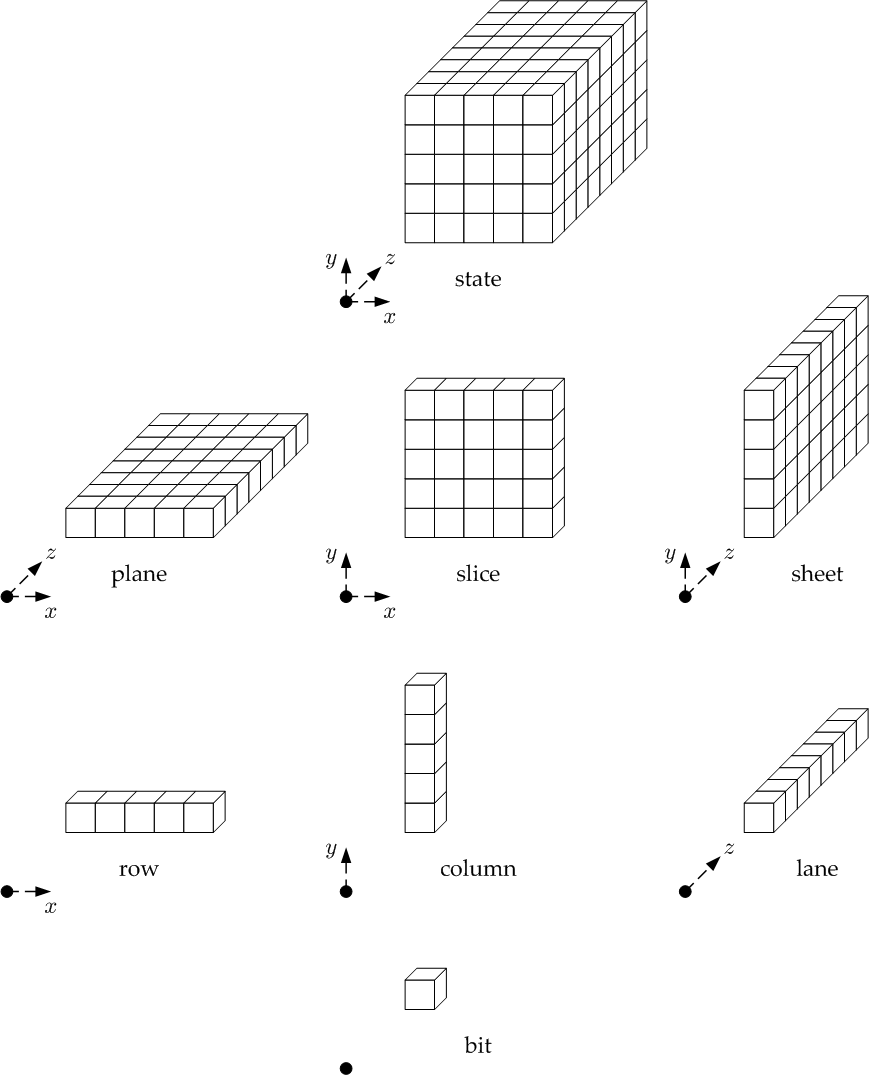
\includegraphics[width=0.7\textwidth]{images/statearray.png}
    \caption{Diagrama do \textit{state array}}
    \label{fig:statearray}
\end{figure}

O uso do \textit{state array} permite que as funções internas sejam definidas
em termos de posições nessa matriz de forma prática. O estado guarda valores
parciais do \textit{hash} e todas as funções internas recebem como parâmetro
o estado atual e retornam como saída o estado atualizado.

O primeiro valor do estado é gerado à partir da mensagem $S$ a ser cifrada, e o
resultado do \text{hash} é o estado após o último passo convertido novamente em
\textit{string}, passos estes que serão explicados nas próximas questões.

\subsection{Como é feita a conversão de \textit{strings} para
    \textit{state array}?}

Seja $S$ uma \textit{string} de $b$ \textit{bits} que representa o estado da
permutação \Keccak-$p[b, n_{r}]$. O \textit{state array} $A$ é definido da
seguinte forma no SHA-3, usando $b = 1600$ e $w = 64$:

Para toda tripla $(x, y, z)$ tal que $0 \leq x < 5$, $0 \leq y < 5$ e
$0 \leq z < w$,

\begin{center}
    $A[x, y, z] = S[w \cdot 5y + w \cdot x + z = S[w \cdot (5y+x) + z]$
\end{center}

Por exemplo, a posição $A[2, 1, 4]$ é obtida do \textit{bit}
$S[64 \cdot (5 \cdot 1 + 2) + 4] = S[772]$ da \textit{string} de entrada.

Usando essa fórmula, os \textit{bits} são mapeados sequencialmente por pista,
coluna e linha, ou seja, os primeiros 64 \textit{bits} serão mapeados na pista
da coluna 0 e linha 0, os próximos serão mapeados na pista da coluna 1 e linha
0, e assim sucessivamente.

É esta característica que gera o tamanho $b$ da string $S$, porque para cada
pista de $w$ \textit{bits}, existem $5 \cdot 5 = 25$ células pelo formato da
matriz, portanto $b = 25 \cdot w$.

\subsection{Como é feita a conversão de \textit{state array} para
    \textit{strings}?}

A conversão inversa, ou seja, de \textit{state array} para \textit{string}, é
feita de forma análoga, concatenando todas as pistas por coluna (gerando os
planos) e então por linha. Utilizando-se da mesma fórmula posicional,

\begin{center}
    $S[w \cdot (5y+x) + z] = A[x, y, z]$ \\
    ou \\
    $S[i] = A[\floor*{i \div (5w)}, \floor*{i \div w \pmod{w}}, i \pmod{w}]$
\end{center}

Primeiro se concatenam os $w$ \textit{bits} de uma pista:

$Lane(i, j) = A[i, j, 0] \concat A[i, j, 1] \concat \cdots \concat A[i, j, w-1]$

Onde $\concat$ denota concatenação de \textit{strings}, de forma que as pistas
da coluna $i = 0$, usando $w = 64$, sejam:

$\begin{array}{c}
    Lane(0, 0) = A[0, 0, 0] \concat A[0, 0, 1] \concat \cdots \concat A[0, 0, 63] \\
    Lane(1, 0) = A[1, 0, 0] \concat A[1, 0, 1] \concat \cdots \concat A[1, 0, 63] \\
    \vdots \\
    Lane(5, 0) = A[5, 0, 0] \concat A[5, 0, 1] \concat \cdots \concat A[5, 0, 63]
\end{array}$

E assim para todas as pistas. A \textit{string} que representa cada plano é a
concatenação de todas as pistas na sua coluna $j$:

$Plane(j) = Lane(0, j) \concat Lane(1, j) \concat \cdots \concat Lane(4, j)$

De forma que os planos de cada uma das colunas $0 \leq j < 5$ seja:

$\begin{array}{c}
    Plane(0) = Lane(0, 0) \concat Lane(1, 0) \concat \cdots \concat Lane(4, 0) \\
    Plane(1) = Lane(0, 1) \concat Lane(1, 1) \concat \cdots \concat Lane(4, 1) \\
    \vdots \\
    Plane(4) = Lane(0, 4) \concat Lane(1, 4) \concat \cdots \concat Lane(4, 4)
\end{array}$

A concatenação destes planos, então, gera a \textit{string} a partir do estado:

$S = Plane(0) \concat Plane(1) \concat \cdots \concat Plane(4)$

No resultado final, a concatenação de todos os \textit{bits} gera a seguinte
\textit{string}:

$S = A[0, 0, 0] \concat \cdots \concat A[0, 0, 63] \concat A[0, 1, 0] \concat \cdots \concat A[0, 4, 63] \concat A[1, 0, 0] \concat \cdots \concat A[4, 4, 63]$

\subsection{Explicar os cinco passos de mapeamento (\textit{step mappings})}

Cada rodada do SHA-3 é composta por cinco passos de mapeamento do \Keccak-$p$,
representados pelas funções $\iota$, $\chi$, $\pi$, $\rho$ e $\theta$, que
recebem como parâmetros posições de \textit{bits}, colunas e linhas e manipulam
o \textit{state array} da operação.

\subsubsection{Função \textit{theta} $\theta$}

A função \textit{theta} é definida pela seguinte fórmula:

$\theta(M[x, y, z]) = M[x, y, z] \oplus \sum\limits_{y'=0}^{4}M[x-1, y', z] \oplus \sum\limits_{y'=0}^{4}M[x+1, y', z-1]$

É uma função de substituição que utiliza os \textit{bits} de colunas adjacentes
e da mesma pista na qual está sendo aplicada. Para cada pista $A[x, y]$, cada
um dos $w$ \textit{bits} $z$ é logicamente somado com um somatório de uma
coluna da linha anterior e com um somatório de uma coluna da linha posterior,
como mostrado na figura~\ref{fig:theta}.

\begin{figure}[ht]
    \centering
    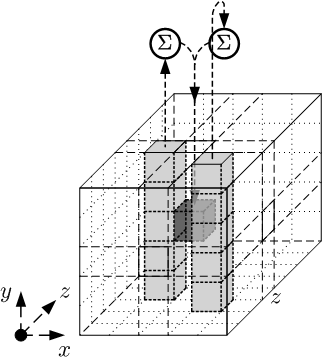
\includegraphics{images/theta.png}
    \caption{Visualização da função theta.}
    \label{fig:theta}
\end{figure}

Dessa forma, cada um dos \textit{bits} do \textit{state array} é afetado por
11 \textit{bits} do estado anterior, sendo 5 de cada coluna utilizada e o
próprio \textit{bit} em que a função foi aplicada. Isso cria um alto grau de
difusão dos efeitos de todas as funções no resultado.

A função \textit{theta} é a primeira porque mistura a parte interna do estado
(invisível para um atacante) com a parte externa, muito por causa do
funcionamento das funções esponja, portanto um atacante não pode acessar a
entrada das funções subsequentes apenas analisando a parte visível do estado.

\subsubsection{Função \textit{rho} $\rho$}

A função \textit{rho} é definida pela seguinte fórmula:

$\rho(M[x, y, z]) = \begin{cases}
    M[x, y, z], \mbox{se } x=y=0 \\
    M[x, y, z - \frac{(t+1)(t+2)}{2}] \mid 0 \leq t < 24 \land
    \begin{pmatrix}0 & 1 \\ 2 & 3\end{pmatrix}
    \begin{pmatrix}0 \\ 1\end{pmatrix} =
    \begin{pmatrix}x \\ y\end{pmatrix}
    \mbox{ em } GF(5)
\end{cases}$

É uma função de permutação que utiliza os \textit{bits} de uma pista $A[x, y]$.
No caso de $(x, y) = (0, 0)$, a função não altera os \textit{bits}, mas para
os outros casos, ela aplica um deslocamento circular dos \textit{bits} como um
embaralhamento dos mesmos, usando o valor $t$ para definir quantos bits será
deslocado, como mostrado na figura~\ref{fig:rho}.

\begin{figure}[ht]
    \centering
    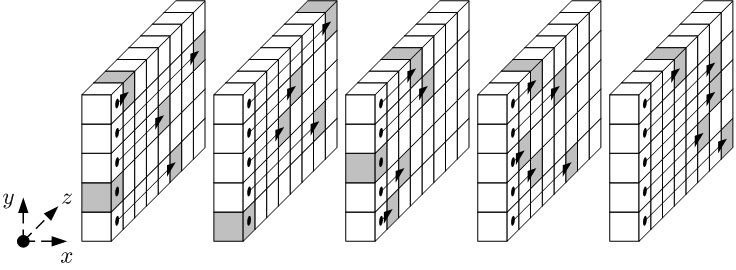
\includegraphics{images/rho.png}
    \caption{Visualização da função rho.}
    \label{fig:rho}
\end{figure}

Essa transformação gera a difusão entre os \textit{bits} de uma mesma pista,
acelerando os efeitos das funções em \textit{bits} próximos da \textit{string}
de entrada e do \textit{state array}, já que as outras funções criam difusão
entre linhas, colunas e pistas, mas não entre \textit{bits}.

\subsubsection{Função \textit{pi} $\pi$}

A função \textit{pi} é definida pela seguinte fórmula:

$\pi(M[x, y]) = M[x', y'] \mbox{ onde }
\begin{pmatrix}x' \\ y'\end{pmatrix} =
\begin{pmatrix}x \\ y\end{pmatrix}
\begin{pmatrix}0 & 1 \\ 2 & 3\end{pmatrix}$

É uma função de permutação que utiliza as pistas. Assim como \textit{theta},
\textit{pi} faz um deslocamento circular usando uma fórmula semelhante, como
mostrado na figura~\ref{fig:pi}.

\begin{figure}[ht]
    \centering
    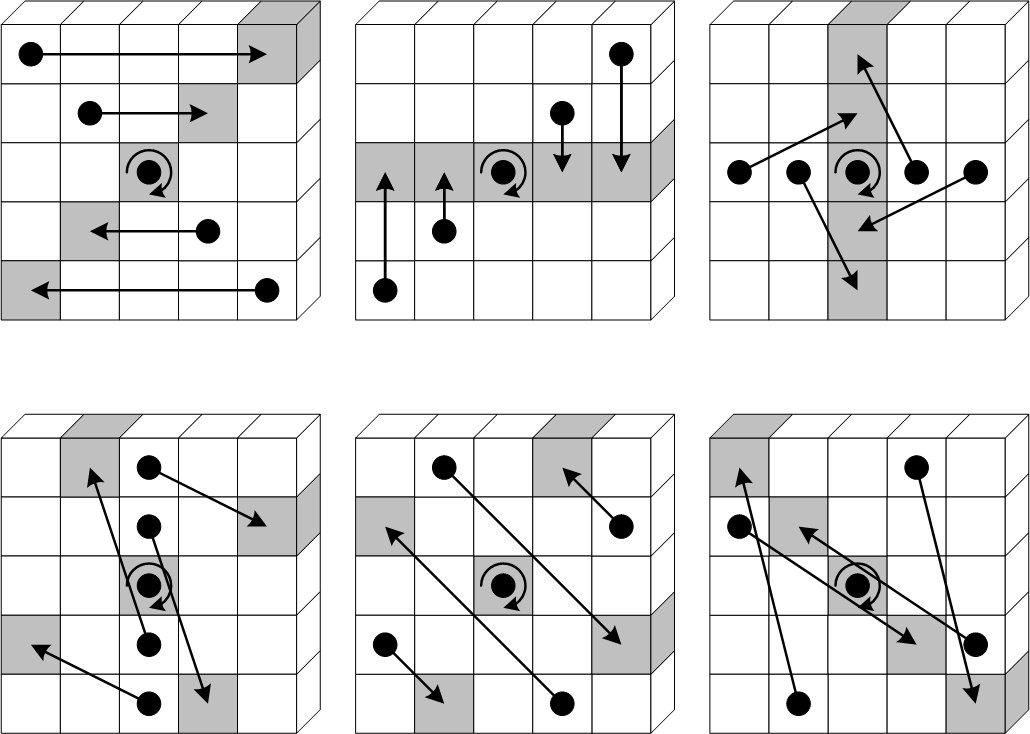
\includegraphics[width=0.7\textwidth]{images/pi.png}
    \caption{Visualização da função pi.}
    \label{fig:pi}
\end{figure}

Essa transformação gera a difusão entre diferentes pistas.

\subsubsection{Função \textit{chi} $\chi$}

A função \textit{chi} é definida pela seguinte fórmula:

$\chi(M[x, y, z]) = M[x, y, z] \oplus (\neg{M}[x+1, y, z] \land M[x+2, y, z])$

É uma função de substituição que utiliza os \textit{bits} posteriores ao
\textit{bit} sendo aplicado, sendo o passo não-linear que torna a função
\Keccak{} uma função irreversível, ou seja, impede a obtenção da pré-imagem a
partir do \textit{hash}. O passo \textit{chi} é mais facilmente visualizado se
usando um circuito digital, como mostrado na figura~\ref{fig:chi}.

\begin{figure}[ht]
    \centering
    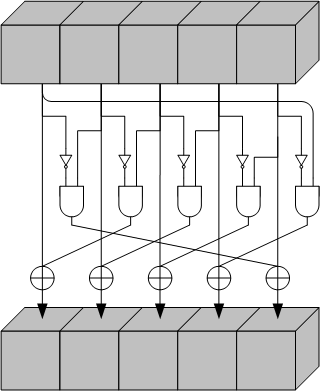
\includegraphics{images/chi.png}
    \caption{Visualização da função chi.}
    \label{fig:chi}
\end{figure}

Sua definição possui propriedades algébricas que garantem que a saída não
possui correlação direta com a entrada em termos de paridade, ou seja, não é
possível concluir nada sobre a entrada analisando a quantidade de \textit{bits}
em 0 ou 1 da saída.

\subsubsection{Função \textit{iota} $\iota$}

A função \textit{iota} é definida pela seguinte fórmula:

$\iota(M[x, y]) = M[x, y] \oplus RC_{i}$

É uma função de substituição baseada em um valor tabelado e diferente para cada
rodada do SHA-3, e é gerado a partir de uma fórmula que utiliza um gerador de
deslocamento linear realimentado (LFSR, na sigla em inglês) em $GF(2)$:

$RC_{i}[2^{j}-1] = (x^{j+7i} \pmod{x^8 + x^6 + x^5 + x^4 + 1}) \pmod{x} \mbox{ para } 0 \leq j \leq \log w$

Dessa forma, não existe relação de simetria entre as diferentes rodadas, porque
sem este passo, todas as rodadas teriam a mesma fórmula e poderiam ser
simplificadas para permitir ataques.

A função \textit{iota} é somente aplicada na primeira linha e coluna, ou seja,
os parâmetros $x$ e $y$ são sempre 0, e seu efeito é difundido para as outras
linhas e colunas através dos passos \textit{theta} e
\textit{chi}~\cite{keccak:2011}.

\subsection{Explicar a permutação \Keccak-$p[b,n_r]$}

Uma função \Keccak-$p[b, n_r]$ é uma generalização das funções de substituição
e permutação \Keccak{} que podem ser usadas pelo SHA-3 e recebe como parâmetros o
comprimento da \textit{string} $S$, que define o tamanho do
\textit{state array}, e o número de rodadas na fase de absorção.

Cada uma das rodadas $R_{i}$ de \Keccak-$p$ consiste na aplicação dos cinco
passos de transformação, vistos na seção anterior:

\begin{center}
    $R_{i} = \iota \circ \chi \circ \pi \circ \rho \circ \theta$
\end{center}

O \textit{state array} na rodada $i$, denominado $S_{i}$, é encontrado pela
seguinte composição de funções:

\begin{center}
    $S_{i} = \iota(\chi(\pi(\rho(\theta(S_{i-1}))), i)$
\end{center}

Onde $j \geq 2l + 12 - n_r$, sendo $l = \log w$, e $i < 2l + 12$. Essa
definição genérica nos permite gerar versões do \Keccak{} para diferentes
tamanhos de palavras $w$, desde que $w = 2^{k}$. É conveniente utilizar $32$ ou
$64$ por ser o tamanho de uma palavra em processadores modernos, e o FIPS 202
define os seguintes parâmetros por padrão:

$\begin{array}{l}
    b \in \{25, 50, 100, 200, 400, 800, 1600\} \\
    n_{r} = 2l + 12, \mbox{ onde } l \in \mathbb{Z}
\end{array}$

\subsection{Descrever o \textit{framework} \textit{sponge construction}}

Funções esponja são uma classe de funções que recebem uma entrada de tamanho
finito qualquer e produzem uma saída com outro tamanho qualquer desejado, sendo
definidas por três parâmetros: um estado $S$, que contém $b$ bits; uma função
$f$ que permuta ou transforma o estado $S$; e uma função de \textit{padding}
$P$~\cite{noekeon:2011}.

Na inicialização, a função $P$ é aplicada na entrada $M$ e dividida em blocos
de $r$ bits. Os $b$ bits do estado $S$ são zerados. A construção da esponja se
dá em duas fases, chamadas de absorção e compressão.

O tamanho $r$ também é chamado de \textit{bitrate}, porque representa a
quantidade de bits da entrada que são consumidos em cada iteração da função
esponja, e o tamanho $c = |S| - r$ é chamado de capacidade, e representa o
nível de segurança atingido pela variante da função - SHA-3, $r + c = b$.

Na fase de absorção, cada bloco $P$ de $r$ bits é combinado com os primeiros
$r$ bits, com os restantes $c$ bits preenchidos com zero, do estado $S$ com
\texttt{xor} e é aplicada a função $f$ no resultado, ou seja,
$S_{i} = f(S_{i-1} \oplus P_{i} \concat 0^{c})$. Ao final de todas as
iterações, ou seja, após a mensagem $M$ ser completamente consumida pela
absorção da esponja, a saída da função $f$ será o \textit{hash} gerado.

Na fase de compressão, os primeiros $r$ bits do estado $S$ são retornados, e
caso mais bits sejam desejados, se aplica novamente a função $f$ em $S$ para
transformar o estado.

\subsection{Explique a família de funções esponja \Keccak}

O algoritmo escolhido como SHA-3 é baseado na família de funções esponja
\textbf{\Keccak}, mais especificamente na variante com 1600 bits de largura da
função de permutação~\cite{fips:2015}.

O \Keccak{} segue a a estrutura dos algoritmos de \textit{hash} comuns, onde os
blocos $P$ da mensagem a ser cifrada vão sendo concatenados alternadamente com
aplicações de uma função de transformação $f$, de forma que a passagem $i$
tenha o seguinte formato:

\begin{center}
        $S_{i} = f(S_{i-1} \oplus P_{i})$
\end{center}

Para que a mensagem seja transformada pela função esponja, ela precisa que uma
função de \textit{padding} $pad$ seja aplicada. O algoritmo utilizado pelo
\Keccak{} para \textit{padding} da entrada se chama $pad10*1$ e é definido por
$pad(M) = b - (|M| \mod b)$, onde $b$ é o tamanho do bloco em \textit{bits}
da esponja e $|M|$ é o comprimeito da mensagem em \textit{bits}.

O resultado $P$ da função $pad10*1$ tem o formato binário
$1 \concat 0^{m-2} \concat 1$, ou seja, $m-2$ zeros cercados por uns.

A função \Keccak[c], onde $c$ define a capacidade da função, é definida por:

\begin{center}
    \Keccak$[c] = Sponge[$\Keccak-$p[1600, 24], pad10*1, 1600-c]$
\end{center}

Ou seja, é uma aplicaçao de função esponja cujo parâmetro $f$, a função de
transformação, é \Keccak-$p$ com 1600 \textit{bits} de estado e 24 rodadas,
utiliza $pad10*1$ como função de \textit{padding} da mensagem e possui bloco
de tamanho $r = 1600 - c$.

A utilização destes parâmetros define \Keccak$[c]$ como uma função que aceita
uma mensagem de tamanho arbitrário, onde cada uma das 24 rodadas processa um
bloco da mensagem de tamanho $r = 1600-c$ e com grau de segurança $c$.

\subsection{Explique a especificação da função SHA-3}

A definição do SHA-3 publicada pelo NIST prevê dois tipos de função baseadas no
\Keccak, funções de \textit{hash} criptográficas e funções de saída extendida
(XOF, ou \textit{extendable output function}), também chamadas de SHAKE.

\begin{enumerate}[label=\roman*.]
    \setlength\itemsep{1em}

    \item Funções de \textit{hash} SHA-3 \newline

        As funções de \textit{hash} podem ser definidas genericamente para um
        tamanho do \textit{hash} gerado $d$ e mensagem $M$ com a seguinte
        fórmula: \newline

        SHA-3$[d](M) =$ \Keccak$[2d](M \concat 01, d)$ \newline

        Observando que os bits $01$ são concatenados à mensagem $M$ antes da
        execução a função. O NIST definiu $d \in \{224, 256, 384, 512\}$ para
        o SHA-3, existindo portanto SHA3-224, SHA3-256, SHA3-384 e SHA3-512:

        \begin{itemize}
            \setlength\itemsep{0.2em}
            \item SHA3-224(M) = \Keccak$[448](M \concat 01, 224)$
            \item SHA3-256(M) = \Keccak$[512](M \concat 01, 256)$
            \item SHA3-384(M) = \Keccak$[768](M \concat 01, 384)$
            \item SHA3-512(M) = \Keccak$[1024](M \concat 01, 512)$
        \end{itemize}

        Estes tamanhos são escolhidos de forma que o SHA-3 seja uma
        substituição do SHA-2, que utiliza os mesmos tamanhos. \newline

        Seria possível, caso desejado, definir tamanhos maiores, como 1024 ou
        2048, provendo um espaço muito maior e diminuindo a quantidade de
        colisões, mas tornando o algoritmo mais lento e diminuindo o grau de
        segurança do \textit{hash}.

    \item Funções de saída extendida (SHAKE) \newline

        As funções XOF podem ser definidas genericamente para uma capacidade
        de segurança $c$ e mensagem $M$ com a seguinte fórmula: \newline

        $SHAKE[c](d, M) =$ \Keccak$[c](M \concat 1111, d)$ \newline

        Observando que os bits $1111$ são concatenados à mensagem $M$ antes da
        execução da função. O NIST definiu $c \in \{128, 256\}$ para o SHAKE,
        existindo portanto SHAKE-128 e SHAKE-256.

        \begin{itemize}
            \setlength\itemsep{0.2em}
            \item SHAKE-128(M) = \Keccak$[128](M \concat 1111, 128)$
            \item SHAKE-256(M) = \Keccak$[256](M \concat 1111, 256)$
        \end{itemize}

        Nota-se que o tamanho da saída, diferente das funções SHA-3, é apenas
        $d = c$, e não $2d$, porque o \Keccak{} pode gerar um comprimento
        infinito de \textit{bits}, e mais podem ser gerados se ''espremendo``
        a esponja.
\end{enumerate}

\subsection{Apresente a análise de segurança}

Os algoritmos de \text{hash} anteriores ao SHA-3, desde o MD4 até o SHA-2,
utilizam o mesmo mecanismo chamado de Merkle-Damgard. Embora seja um método
provadamente eficiente e seguro, o uso do mesmo mecanismo significa que uma
quebra de outro algoritmo como o SHA-1 também se torna uma ameaça em potencial
ao SHA-2, até então o algoritmo mais seguro.

Um ataque de força bruta ao SHA-1 tem custo de $2^{80}$, mas já existem ataques
que reduzem essa complexidade para $2^{58.5}$, o que é um custo factível para
computadores modernos. Apesar de o único ataque prático já realizado contra o
SHA-2 ainda ter um custo absurdo de $2^{253.6}$, os ataques realizados em
outros algoritmos podem também encontrar brechas no SHA-2~\cite{dobbs:2013}.

Na competição que escolheu o SHA-3, houve condições para os competidores para
evitar que ataques conhecidos pudessem ser explorados nos algoritmos, e um dos
requisitos era não utilizar o mecanismo de Merkle-Damgard, motivo pelo qual o
\Keccak utiliza a construção de esponja.

Além disso, enquanto o nível de segurança de Merkle-Damgard é ligado ao tamanho
da saída - N/2 \textit{bits} de segurança contra colisão e N \textit{bits} de
segurança contra pré-imagem -, a construção de esponja tem um tamanho da saída
variável e um núvel de segurança controlado pela capacidade da esponja.

Portanto, a segurança adicional do \Keccak se dá pelo seu formato diferente,
resistente aos ataques conhecidos atualmente, e pela sua capacidade de
modificação do parâmetro de segurança conforme desejado. Os tamanhos definidos
pelo NIST provêm a mesma resistência à pré-imagem, segunda pré-imagem e colisão
que o já existente SHA-2.

\subsection{Exemplos}

\begin{itemize}
    \item SHA3-224("segurança em computação") \newline
        \texttt{87 0B D5 50 EB 20 44 45 22 AF 19 1A A0 DA 03 CC 11 FB 76 92 70 B2 4F DA BB 64 6F EC} \newline
    \item SHA3-256("segurança em computação") \newline
        \texttt{B1 CB C2 AF 9D 81 58 B2 32 DE 7B C0 88 C0 48 E1 F9 0F 7F E2 65 6C 76 A1 AB 44 0A EF 46 EF DF 2E} \newline
    \item SHA3-384("segurança em computação") \newline
        \texttt{B7 9C D7 EE 92 2B 78 A3 D5 CB D2 2E 4C 75 69 42 AE 10 86 07 78 D4 BD 90 2E A3 EE 74 38 D1 CD 26 C0 B2 58 06 14 20 89 FB 85 71 07 29 BE 94 26 AB} \newline
    \item SHA3-512("segurança em computação") \newline
        \texttt{C9 AC B8 EE F9 8F 4A 4D 11 75 DC 5B 3B CF C9 83 D8 AB C7 88 6E 90 27 C7 8A 6F E6 91 57 0F CE F9 26 10 79 1E 1E DF 00 5C D6 12 98 0E 2D 71 5E 43 CD E9 CE 4F 68 59 BE B5 30 14 D3 4D 64 67 EB 28}
\end{itemize}

\let\thesubsection\oldsubsection%
